\documentclass[pract, och, master]{SCWorks}
%    spec
%    bachelor
%    master
%    och
%    zaoch
%    referat
%    coursework
%    diploma
%    pract
%    pract
%    autoref
%    assignment
%    review
%    critique
%    times
%    nir
\usepackage[T2A]{fontenc}
% \usepackage[cp1251]{inputenc}  %NOTE: uncomment to compile .tex with windows
\usepackage[utf8]{inputenc} %NOTE: comment to compile .tex with windows
\usepackage{graphicx}
% \usepackage[sort,compress]{cite}
\usepackage{amsmath}
\usepackage{amssymb}
\usepackage{amsthm}
\usepackage{fancyvrb}
\usepackage{longtable}
\usepackage{array}
\usepackage[english,russian]{babel}
\usepackage{tempora}
\usepackage[colorlinks=true]{hyperref}


% \usepackage{biblatex}
% \bibliography{thesis} 
% \bibliographystyle{gost2003}  

% \usepackage[
% backend=bibtex,
% %  style=gost2003,
% sorting=ynt
% ]{biblatex}
% \addbibresource{thesis.bib}

% \usepackage[backend=biber,style=ieee]{biblatex}
% \addbibresource{thesis.bib}

\newcommand{\eqdef}{\stackrel {\rm def}{=}}

\newtheorem{lem}{учебная (Научно-исселдовательская работа)}

\begin{document}

\chair{информатики и программирования}
\title{Разработка системы траекторного управления БПЛА}
\course{1}
\group{173}
%\department{}
\napravlenie{02.03.02 "--- Математическое обеспечение и администрирование информационных систем}
\author{Ворониной Екатерины Юрьевны}
\chtitle{доцент кафедры ИиП}
\chname{Е.В. Кудрина}
\satitle{Кандидат ф.-м.наук, доцент}
\saname{М.В. Огнева}
\term{1}
\practtype{производственная ("Научно-исследовательская работа")}
% \duration{2}
\practStart{01.09.2023}
\practFinish{14.01.2024}
\date{2024}

\maketitle

\tableofcontents

\abbreviations
\begin{description}
	\item БПЛА --- беспилотный летательный аппарат;
	\item СТУ --- система траекторного управления;
	\item НПУ --- наземный пункт управления;
	\item АУ --- бортовая аппаратура управления;
	\item НАУ --- наземная аппаратура управления;
	\item БАС --- беспилотная авиационная система;
	\item АПИК --- аналитическая программно-инвариантная конструкция;
	\item СВС --- система воздушных сигналов;
	\item ВПП --- взлетно-посадочная полоса;
	\item БТС --- беспилотная транспортная система;
	\item МЭМС --- микроэлектромеханические системы
	\item GPS --- Global Position System (Глобальная система позиционирования);
	\item ГЛОНАСС --- Глобальная навигационная спутниковая система;
\end{description}

\intro
Развитие беспилотной авиации входит в область интересов государственной промышленной политики. 
В связи с тем, что  Правительство РФ утвердило стратегию развития беспилотной авиации до 2030 г. \cite{goverment} 
и на перспективу до 2035 г., в настоящее время сфера беспилотной авиации получает большую финансовую поддержку со стороны государства.

Нарастающий интерес к беспилотной авиации тенденция также и общемировая. Это происходит по ряду 
причин. БПЛА, как правило, гораздо дешевле пилотируемых самолетов и вертолетов. Дешевле, чем 
подготовка летчика, обходится и подготовка оператора беспилотной системы. Отсутствие пилота 
позволяет исключить бортовые системы жизнеобеспечения, уменьшить массу и габариты БПЛА, 
а также увеличить диапазон допустимых перегрузок и влияющих факторов. Большое значение имеет 
и фактор безопасности, поскольку потери беспилотных аппаратов не ведут к потере пилотов.

Большой рост количества разработок БПЛА именно в последнее десятилетие не случаен. Этому 
способствовали определенные объективные предпосылки, указанные в работах \cite{uvDev,kbpa}, которые созрели именно к этому времени. 
Они связаны с серьезными технологическими успехами в различных областях. Например, этому 
способствовало:
\begin{enumerate}
	\item появление легких и прочных композитных материалов;
	\item развитие микроэлектронной компонентной базы: микроконтроллеров, микросистемных навигационных 
	датчиков, приемопередатчиков радиосигналов, различных СВЧ-устройств, микроэлектронных драйверов 
	сильноточных потребителей, миниатюрных видеокамер;
	\item появление и быстрое развитие высокоэффективных возобновляемых источников питания на основе 
	литий-полимерных аккумуляторов, топливных элементов;
	\item разработки в области высокоресурсных бесколлекторных электродвигателей, а также 
	реактивных и поршневых двигателей;
	\item развитие спутниковых систем глобального позиционирования;
	\item общее развитие вычислительной техники, включая появление специальных операционных систем, 
	интерфейсов, математического и алгоритмического обеспечения;
\end{enumerate}

Проблема синтеза САУ БПЛА как задачи автоматизации управления движением БПЛА была и остается на переднем крае в 
общем комплексе проблем создания БПЛА \cite{kbpa}. Для управления траекторией движения беспилотного летательного судна, 
САУ необходимо решать ряд задач, связанных с планированием и реализацией сложных пространственных движений. К этому ряду относится 
задача нахождения допустимого пути летательного аппарата в трехмерном пространстве, огибающего статические препятствия, 
а также связанные с ней задачи путевой и траекторной стабилизации. 
Для решения перечисленных задач, необходимо как можно более точно оценивать положение и ориентацию БПЛА в режиме реального времени. 
Возрастающая с ростом количества бортовых датчиков сложность системы оценки, а также нарастающая со временем погрешность данных измерений 
бортовых сенсоров приводит к необходиомсти применения алгоритмов фильтрации и регуляторов.   


Целью данной работы является 
% разработка математической модели движения БПЛА и 
анализ подходов к решению задачи системы траекторного управления роторным БПЛА. 
Исходя из цели определены следующие задачи:
\begin{itemize}
	\item классификация БПЛА;
	% \item моделирование структуры системы управления БПЛА;
	\item исследование современных подходов к конструкции бортовой системы БПЛА;
	\item анализ алгоритмов построения траектории движения ЛА и обработки данных с бортовых сенсоров;
\end{itemize}
 
% ОСНОВНАЯ ЧАСТЬ
\section{Классификация и бортовое устройство БПЛА}

Приведенные ниже термины, касающиеся описания устройств БПЛА были заимствованы из работ \cite{uavAvia,kbpa}.

Летательным аппаратом называется техническое устройство, предназначенное для осуществления полетов в земной 
атмосфере или в космосе. По наличию экипажа все ЛА можно разделить две группы: пилотируемые и беспилотные.

Под термином беспилотный летательный аппарат понимается ЛА, не имеющий на борту экипажа и способный перемещаться 
в воздухе в автономном режиме, посредством дистанционного управления, оператором с НПУ или сочетанием указанных 
способов. Дистанционное управление БПЛА может осуществляться с помощью дискретных разовых радиокоманд. 
В автономном режиме оператор осуществляет функцию контроля.

В основу классификации БПЛА могут быть положены признаки, характеризующие конструктивные особенности, 
способы управления,  массовые и габаритные параметры. Конструктивно БПЛА разделяются на роторные --- с 
вращающимся крылом и самолетные --- с неподвижным. На рисунке ~\ref{classification} приведена более подробная классификация беспилотных ЛА.

\begin{figure}[h]
	\centering
	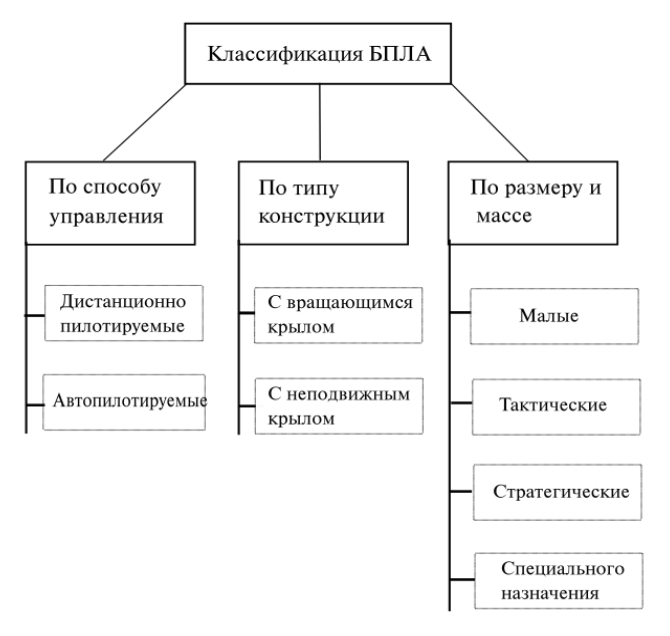
\includegraphics[width=11cm]{img/uav_classification.png}
	\caption{\label{classification}%
	Классификация БПЛА}
\end{figure}

Подъемная сила у БПЛА самолетного типа создается  аэродинамическим способом за счет напора воздуха, набегающего под неподвижное крыло. 
Судна самолетного типа, как правило, отличаются большей, в сравнении с роторными, длительностью полета, большей максимальной высотой полета и высокой скоростью. 
Но в отличии о роторных моделей, из-за особенностей конструкции, самолетные БПЛА не способны зависать в воздухе. Также приемущества роторной модели, 
отмеченные в \cite{}, это возможность свободного полета в трех плоскостях, в том числе назад, отсутствие необходимости в специализированных 
взлетно-посадочных площадках и перевозка груза на внешнем подвесе.

Мультикоптер --- это роторный БПЛА, имеющий более двух несущих винтов. Подъемная сила у роторных БПЛА создается силами моментов 
несущих винтов, расположенных параллельно земле. Реактивные моменты уравновешиваются за счет вращения несущих винтов попарно в разные стороны или наклона вектора 
тяги каждого винта в определенном направлении.

Квадрокоптер --- это четырехроторный БПЛА, приводящийся в движение четырьмя несущими винтами, расположенными в одной плоскости параллельно земле. 
Данный тип конструкции БПЛА  наиболее распространен в сфере гражданской беспилотной авиации по причине сравнительной простоты конструкции и управления.
Существуют две схемы квадрокоптера: 
\begin{itemize}
	\item $+$, где один из роторов является передним, а противоположный ему задним. Два оставшихся ротора являются боковыми;
	\item $x$, где передними являются одновременно два ротора, а два других задними;
\end{itemize}

% На рисунке ~\ref{drone} приведен механизм движения квадрокоптера.

% \begin{figure}[!ht]
% 	\centering
% 	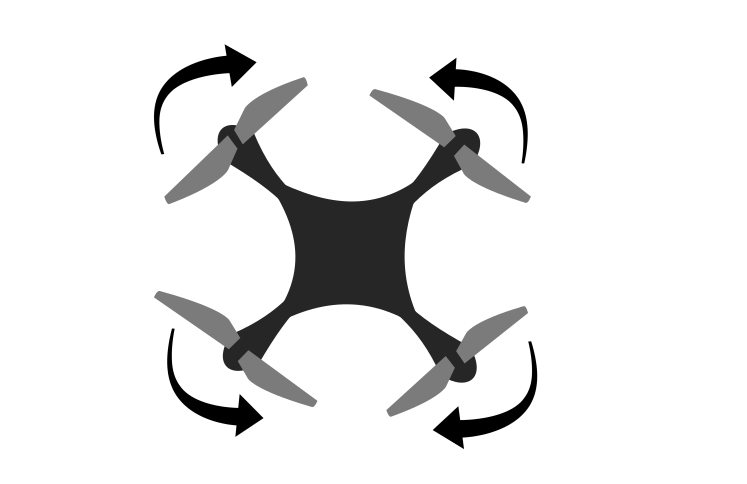
\includegraphics[width=6cm]{img/drone pic.png}
% 	\caption{\label{drone}%
% 	Механизм движения квадрокоптера}
% \end{figure}

\section*{Бортовое устройство БПЛА}

Основным компонентом комлпекса САУ БПЛА является электронная система управления, называемая летным контроллером. 
Структура САУ описана в работе \cite{ShilovMFTI}, где автор перечисляет следующий набор компонентов:
\begin{itemize}
	\item процессор и/или микроконтроллер с модулями оперативной и энергонезависимой памяти, необходимые для функционирования систем БПЛА;
	\item модуль определения пространственного положения, состоящий из многоосевых МЭМС-сенсоров, таких как гироскопы, акселерометры и магнетометры;
	\item модуль высотометрических датчиков, для определения высоты и воздушной скорости;
	\item модуль приема спутниковой навигации GPS, для точного геопозиционирования;
	\item модуль радиосвязи, для ручного управления и передачи данных телеметрии;
\end{itemize}

С целью уменьшения помех высотометрических, спутниковых и датчиков пространственного положения применяются алгоритмы фильтрации Калмана и ПИД-регуляторы, суть которых 
подробно изложена в \cite{filter}.

Наряду с основным объектом комплекса --- САУ, которая обеспечивает 
автономность полета летательного аппарата, в бортовую систему летательного аппарата также входят:
\begin{itemize}
	\item приемник радиосигнала, принимающий сигнал передатчика для осуществления ручного управления аппаратом;
	\item контроллеры двигателей, которые принимают входной сигнал широтно-импульсной
	модуляции от системы управления и устанавливают заданный режим работы каждого из двигателей;
	\item  литий-полимерный аккумулятор для питания двигателей и DC-DC преобразователей, встроенных в контроллеры двигателей для
питания системы управления и приемника радиосигнала;
\end{itemize}
  
В \cite{uvDev} отмечается, что базовая система управления БПЛА часто дополняется такими компонентами, 
как радиолокационные системы, лидары, ультразвуковые датчики расстояний, камеры и системы 
стабилизации фото и видеооборудования. Данные устройства относятся к системам полезной
нагрузки и не являются обязательными и достаточными для полета БПЛА.


\subsection*{Датчики пространственного положения}

Введем понятия, определяющие характер движения БПЛА.

Крен --- это отклонение плоскости симметрии ЛА от вертикального положения. 
Характеризуется углом крена и скоростью крена. Манёвры крена используются, например, при разворотах, при выполнении фигур пилотажа, при заходе на посадку 
для парирования, смещения траектории летательного аппарата относительно оси взлётно-посадочной полосы. Управление креном БПЛА самолетного типа 
осуществляется элементами механизации крыла. Маневры роторных ЛА осуществляются путем изменением скорости вращения винтов. 

Тангаж --- угловое движение ЛА, при котором его продольная ось изменяет свое направление относительно горизонтальной плоскости. Характеризуется углом тангажа 
и скоростью тангажа. Маневры авиамодели с увеличением угла тангажа называются кабрированием, а с уменьшением --- пикированием. Эти манёвры  для моделей самолетного 
типа осуществляются созданием момента тангажа за счет отклонения таких органов управления как руль высоты и элевонов. 

Рыскание --- угловые движения ЛА вокруг вертикальной оси.

Механизм движения квадрокоптера изображен на рисунке \ref{drone_run}.

\begin{figure}[!ht]
	\centering
	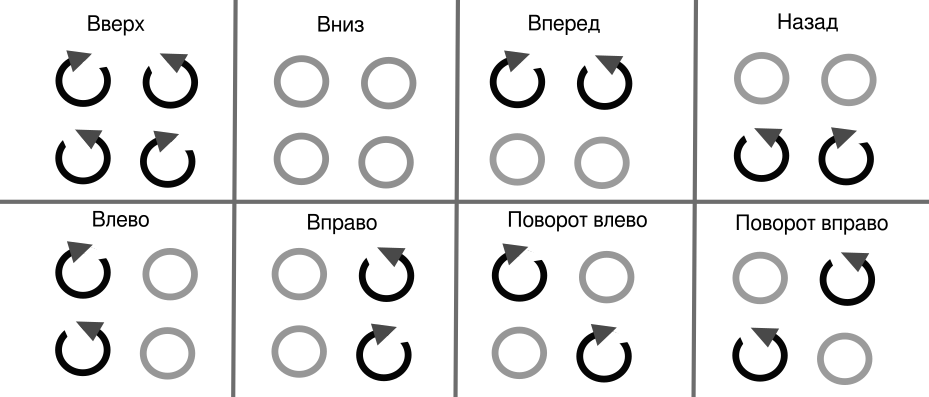
\includegraphics[width=14cm]{img/uavRun.png}
	\caption{\label{drone_run}%
	Механизм движения квадрокоптера}
\end{figure}


Акселерометр --- это прибор, измеряющий проекцию кажущегося ускорения, то есть разности между истинным ускорением объекта и гравитационным ускорением. 
По конструктивному исполнению акселерометры подразделяются на однокомпонентные, двухкомпонентные, трёхкомпонентные. Соответственно, они позволяют 
измерять ускорение вдоль одной, двух и трёх осей. Принцип работы акселерометров основан на измерении смещения инерционной массы относительно корпуса 
и преобразовании его в пропорциональный электрический сигнал.

Гироскоп предназначен для определения угловых скоростей БПЛА. Это навигационный прибор, основным элементом которого является быстро вращающийся ротор, закрепленный так, 
что ось его вращения может поворачиваться. Оси поворота устройства ограничены пружиной, так что, во время выполнения ЛА разворота, гироскоп будет деформировать 
пружину, пока не уравновесится момент внешней силы. В этом случае сила сжатия или растяжения пружины пропорциональна угловой скорости движения летательного аппарата.

Пирометр – оптический прибор, измеряющий температуру тел без непосредственного 
контакта. В авиации используется устройство пирогоризонт, состоящее из из двух 
пар пирометрических датчиков, расположенных под углом 90 градусов. 
Если модель летит горизонтально, каждый датчик «видит» 50\%
небосвода и 50\% земли. Показания диаметрально противоположных датчиков равны, то есть: 

\begin{align}
    Dat_1 - Dat_3 &= 0,\\
    Dat_2 - Dat_4 &= 0
\end{align}

 

Для вычисления углов крена и тангажа необходимо знать рассогласование, 
возникающее, когда датчики видят 100\% неба и 100\% земли. Для этого необходимо 
на земле, перед вылетом, разместить модель вертикально по крену и тангажу, и 
зафиксировать показания  датчиков в этих положениях. Тогда углы крена и тангажа 
могут быть вычислены по формулам [13, 14]: 

\begin{align}
\gamma = \dfrac{(D_1 - D_3) * 90 }{D_1 - D_3}, \\ \theta = \dfrac{(D_2 - D_4) * 90}{D_2 - D_4}, где
\end{align}

$D_x, x\in [0, 4]$ --- показатель соответсвующего пиродатчика.
 
$\gamma$ --- угол крена.

$\theta$ --- угол тангажа.

\subsection*{Высотометрические датчики}

Высотой полета называется расстояние до самолета, отсчитанное по вертикали от некоторого уровня, принятого за начало отсчета. 
По уровню начала отсчета, как указано в \cite{uavAvia}, различают следующие высоты полета как показано на рисунке \ref{baromMeasure}: 
\begin{itemize}
	\item истинную, отсчитываемую от уровня местности, над которой пролетает самолет;
	\item относительную, отсчитываемую от некоторого условного уровня например, уровня аэродрома;
	\item высоту эшелона, отсчитываемую от уровня с давлением 760 мм.рт.ст; 
	\item абсолютную, отсчитываемую от уровня моря;
\end{itemize}

\begin{figure}[!ht]
	\centering
	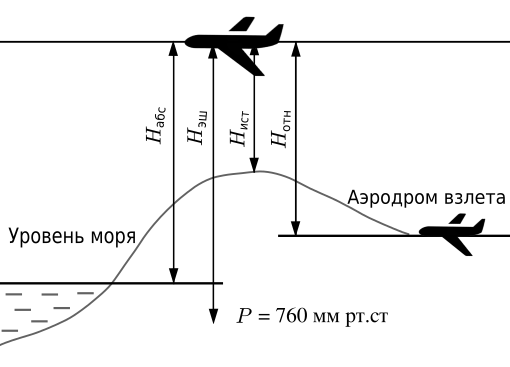
\includegraphics[width=12cm]{img/baromMeasure.png}
	\caption{\label{baromMeasure}%
	Классификация высот полета по уровню начала отсчета}
\end{figure}

Барометрический высотомер --- прибор для измерения давления атмосферного воздуха. Барометричекий метод измерение высоты 
основан на закономерном изменении атмосферного давления и высоты. ПРибор используется для измерения фбсолютной, относительной высоты определенного эшелона. 

% Для нахождения закономерности в атмосфере выделяется 
% вертикальный столб воздуха постоянного сечения $F$ как показано на рисунке \ref{barom}. 

% \begin{figure}[!ht]
% 	\centering
% 	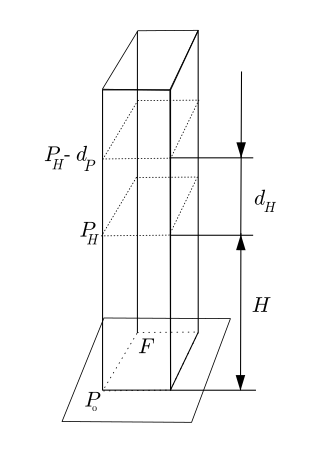
\includegraphics[width=6cm]{img/barom.png}
% 	\caption{\label{barom}%
% 	К выводу формулы барометрического метода измерения высоты}
% \end{figure}

% Давление воздуха у Земли обозначается через $P_0$, а на высоте через $P_H$. 
% При изменении высоты на $d_H$ атмосферное давление уменьшится на величину $d_P$, равную весу $d_Q$ элементарного объема воздуха $d_V$, 
% поделенному на площадь его основания $F$: 

% $d_P = \dfrac{d_Q }{F}$

% Вес $d_Q$ равен произведению объема $d_V$ на удельный вес воздуха $g$ в данном слое. Учитывая, что 

% $d_Q = g*F*d_H$

% Получается следующее соотношение:

% $d_P = -g*d_H$

% Из уравнения состояния газа удельный вес можно выразить через давление $P$, 
% газовую постоянную сухого воздуха $R = 29,27 м/град$ и абсолютную температуру $T$:

% $g = \dfrac{d_P }{R*T}$

% Отсюда получим дифференциальное уравнение следующего вида:

% $\dfrac{d_P}{P} = - \dfrac{d_H}{R * T}$

% Для тропосферы зависимость температуры воздуха от высоты будет иметь следующий вид:

% $T_H = T_0 - tr * H $, где 

% $Т_0$ --- абсолютная температура воздуха у Земли; 
% $tг$ --- вертикальный температурный градиент, град/м; 
% $H$ --- высота, м.;

% Проинтегрировав в левой части от $P_0$ до $P_H$, в правой - от $0$ до $H$, выражается $H$:
% $\[\int_{P_0}^{P_H} \dfrac{1}{P},dP \] = \dfrac{-1}{R} * \[\int_{0}^{H} {\dfrac{1}{T_0 - t_{тр} * H}}, dH \]$

% откуда

% $ \ln{\dfrac{P_H}{P_0}} = \dfrac{1}{R * t_тр} * \ln{\dfrac{T_0 - t_тр * H}{T_0}}$

% Решив это уравнение, закон изменения P_H выразится формулой:

% $P_H = P_0 * (1 - \dfrac{t_тр * H}{T_0})^(\dfrac{1}{R * t_тр})$

% Эта формула называется барометрической. Она выражает зависимость давления от высоты в тропосфере.

Радиометрический высотомер --- прибор, предназначенный для измерения истинной высоты полета, путем подсчета времени прохождения радиосигнала от антенны на воздушном судне 
до поверхности и в обратную сторону. Передатчик радиовысотомера формирует колебания, которые с помощью передающей антенны направляются в сторону земной поверхности. 
Отраженный сигнал поступает на приемную антенну и приемник. Измеритель высоты вырабатывает напряжение, пропорциональное времени прохождения сигнала до земной 
поверхности и обратно, пропорциональное истинной высоте. Отраженные от земли частотно-модулированные высокочастотные колебания принимаются приемной антенной 
радиовысотомера и поступают на вход балансного декодера с запаздыванием по отношению к прямому сигналу на время:
 
\begin{align}
	t = \dfrac{2*H}{c}, где 
\end{align}

$H$ --- высота полета;

$c$ --- скорость света;

%% РЕШЕНИЕ ЗАДАЧИ ТРАЕКТОРНОГО УПРАВЛЕНИЯ 
\section{Программно-алгоритмическе обеспечения САУ БПЛА}

Описанный в работе \cite{Tkachev} подход к траекторному управлению движением БПЛА требует решения задач нахождения допустимого пути и траекторной стабилизации. 
Задачу нахождения допустимого пути автор предлагает решать в два этапа: сперва формировать набор путевых точек в пространстве. Для решения подойдут алгоритмы описанные в 
публикации \cite{Yakovlev}:
\begin{itemize}
	\item алгоритмы на графах: A* \cite{minPathA}, Theta* \cite{theta}, R*\cite{R}, JPS \cite{JPS};
	\item методы случайных деревьев \cite{motionPlanning, treeRRT};
\end{itemize}
 
Получив набор путевых точек с помощью одного из перечисленных выше алгоритмов, вторым этапом следует построить параметрическую кривую 
требуемой степени гладкости \cite{Bestaoui, Shanmugavel, Pan}, которая будет рассматриваться в качестве пути следования ЛА. В момент реализации ЛА выстроенного маршрута, 
возникает проблема распознавания и преодоления возникающих на пути препятствий \cite{Gonoblev}. Решение этой проблемы является ключом к созданию алгоритмов навигации 
БПЛА в пространстве. Представленные в литературе решения \cite{Shirokov, Mystafaev, Gerasuto} для ориентации в пространстве чаще всего основаны на следующих принципах:
\begin{enumerate}
	\item использование систем глобального позиционирования (GPS, ГЛОНАСС) и привязка к карте местности (SLAM);
	\item использование систем машинного зрения в оптическом диапазоне электромагнитного излучения (инфракрасные камеры, стандартные камеры в видимой области спектра);
	\item использование разного рода датчиков расстояния.
\end{enumerate}

Основная проблема, возникающая при использовании систем на основе первых двух принципов --- высокая вычислительная нагрузка, связанная с задачами обработки
изображения от одной или нескольких камер, а также проблема анализа соответствия текущих координат препятствиям, отмеченным на карте местности. Кроме того, системы
глобального позиционирования, как правило, имеют значительную погрешность в локальных условиях, а в закрытых помещениях и вовсе могут не работать, что приводит к
необходимости оборудования последних специальными средствами локализации (активные маяки, метки).

Не смотря на представленные недостатки применение таких подходов для задач наземной робототехники вполне оправданно. Однако для беспилотных летательных аппаратов,
поставленных в жёсткие рамки по массогабаритным показателям и показателям энергоёмкости вычислительной и управляющей систем, скорее подходит третий принцип. В
такой ситуации значение имеет использование датчиков, позволяющих только определить наличие препятствия на пути движения, а задачей распознавания объектов вполне может
заниматься мощная удалённая рабочая станция. Более того эта способность является критически важной в случае сложной картины местности и особенно в условиях
ограниченного пространства. Большое расстояние от оператора, задержки и неточности в управлении увеличивают вероятность возникновения ошибки пилотирования. Для того
чтобы избежать этих проблем, БПЛА на основе данных системы обнаружения препятствий должен самостоятельно принять решение о преодолении или огибании препятствия,
непосредственно вмешиваясь в контур удалённого управления.

% ФИЛЬТР КАЛМАНА ПД РЕГУЛЯТОР 



% \section{Динамичсекая система движения БПЛА}
% Для рассмотрения задачи траекторного управления БПЛА следующие системы координат.
% Связанная система координат (ССК) с началом в точке O центра масс пассивного КА, оси
% которой направлены по главным центральным осям инерции КА и имеют следующие обозначения
% ния: OX – продольная ось, OY – нормальная ось и OZ – поперечная ось

% Лучевая система координат с началом в центре масс пассивного КА. Базовая ось на
% правлена все время по вектору относительной дальности (линии визирования, соединяющие
% центры масс сближаемых КА), а две другие взаимно ортогональные оси и лежат в
% плоскости, перпендикулярной линии визирования.

% Положение БПЛА в пространстве определяется 6 степенями свободы: координатами $(x, y, z)$ и углами ориентации $(ϕ, \theta, ψ)$, 
% в качестве которых рассматриваются углы относительно горизонта $ϕ$, $θ$ и азимутальный угол $ψ$.
% Для обозначения углов ориентации БПЛА $(ϕ, \theta, ψ)$, используются авиационные термины соответсвенно: крен, тангаж и рыскание \cite{uavAvia}. 
% На рисунке \ref{drone_position}

% \begin{figure}[!ht]
% 	\centering
% 	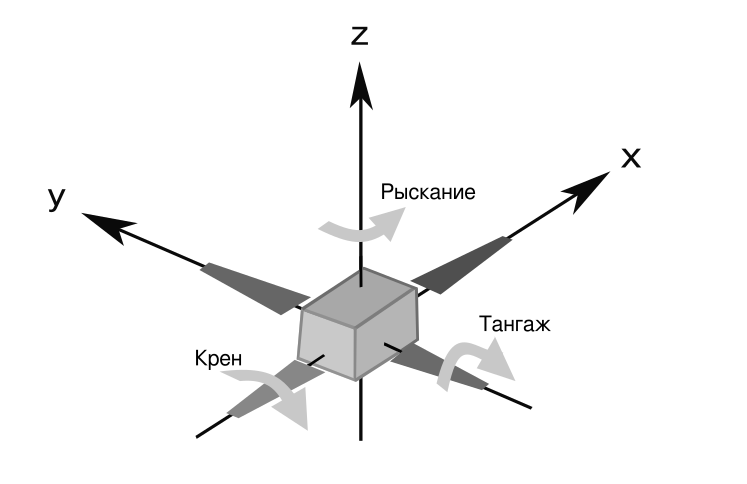
\includegraphics[width=6cm]{img/Navigate SCHEME.png}
% 	\caption{\label{drone_position}%
% 	Характеристики движения ЛА в пространстве}
% \end{figure}

% Для расчета траектории движения БПЛА целесообразно использовать траекторную систему координат: $OX_т$, $OY_т$, $OZ_т$. 
% Траекторная система координат является подвижной, ее начало помещается в центре масс летательного аппарата. 
% Ось $OX_т$ направлена по касательной к траектории БПЛА и совпадает с вектором скорости. Ось $ОY_т$ параллельна земной поверхности. 
% Для оценки параметров движения БПЛА выбираются траекторная OXт, OYт, OZт и нормальная системы координат, лучевая система координат OXл, ОYл, ОZл
% и нормальная система координат в радиолокационной станции (РЛС).


 

% Дроны оснащены встроенным программным обеспечением, которое отправляет команды исполняющим
% устройствам БПЛА или удалённому контроллеру.
% Во многом качество и надежность системы управления БПЛА зависит от программного обеспечения.
% В последние годы для управления роботизированными системами, в том числе и БПЛА, широкое распространение получили операционные системы реального времени (ОСРВ). Такие операционные системы
% позволяют реагировать БПЛА на возникающие события и изменения в окружающей обстановке с высокой скоростью. Применение ОСРВ позволяет полностью
% автоматизировать функционирование БПЛА, оператор
% в данном случае лишь задает полетное задание и выполняет задачи, не связанные с контролем за полетом,
% например, производит аэрофотосъемку, топографическую съемку и т.д.


% Устройство стандартного дрона вертолетного типа
% (квадрокоптер) и основные узлы БПЛА представлены
% на рисунке 

% Как видно из приведенной схемы отличие различных
% типов дронов заключается в аэродинамической схеме
% (вертолетный, самолетный типы, БПЛА вертикального
% взлета и посадки и т.п.). Электронно-механические системы управления как правило различаются не значительно и только в части полезной нагрузки (дополнительного оборудования)


% Hight Definition (HD) maps — карты с точным месторасположением объектов в векторном формате. 
% Они содержат детали, которых нет на обычных картах: знаки, светофоры, разметку, столбы, 
% даже кусты, если это необходимо для навигации.

% Первая подсистема отвечает за извлечение важной информации из необработанных данных, 
% полученных сенсорами, и обеспечивает исследование роботом окружающей среды, на чем в 
% дальнейшем строится принятие решений относительно его будущих действий. Клиентские системы 
% объединяют алгоритмы первой подсистемы, тем самым позволяя им работать в режиме реального
% времени и обеспечивая надежность. Например, если камера генерирует данные
% с частотой 60 Гц, клиентским системам необходимо убедиться, что самый длинный этап 
% обработки занимает менее 16 мс. Платформа облачных вычислений отвечает за автономные 
% вычисления и хранение данных. С ее помощью мы можем тестировать новые алгоритмы, 
% обновлять HD-карты и обучать БТС более качественным моделям распознавания, 
% отслеживания и принятия решений.
  
\conclusion
В ходе работы было выполнено:
\begin{itemize}
    \item это
    \item и это
\end{itemize}

% \printbibliography[title = Reference List]

\bibliographystyle{gost780uv} % стиль цитат
\bibliography{thesis} % источник цитат

\end{document}
